\chapter{Evaluation}\label{chapter:eval}
In previous chapters, we introduced the design and implementation of 2 prototype
video recommendation applications, MiRec and DiRec, that are developed for the
purpose of testing the effect of distributing the UI of a single user recommender system on the users'
experience; whether this distribution will enrich and facilitate users'
experiences of such systems or would be considered redundant or confusing. To
put this to test, we designed a closed user study, in which participants were
asked to interact with and use both prototype applications, and then give their
feedback evaluation through a user experience survey directly after they are done with
using the apps. In this sections, we explain the different phases of the user
study. We also explain our evaluation method, as well as present the results of
the analysed user experience survey collected from the study participants.

\section{User Study Phases}
The overall goal of the study is to elicit the users’ direct
feedback and impressions of their experience of using the prototype apps.
Each of the phases described below will have its own sub-goal that works
towards this main goal. The study is divided into 3 phases. It starts in a
usability demo in which we demonstrate to participants how to use the apps,
which we thought is necessary to avoid any confusion which might affect the
users rating of the app and tamper with their evaluations. Phase 2 is the actual
user test in which participants interact and use the apps. And the final phase
is the post-experiment user experience survey which is done shortly after phase
2. In the course of 2 weeks, participants were invited to use our apps and give
their feedback. We started our evaluation of the collected user feedback shortly
after we had sufficient number of participants that lead to a stable evaluation.
The following are details of each phase of the study as well as a presentation
of the results and how we interpret them.
\subsection{Phase 1: Usability Demo}
The goal of this phase is to explain clearly to participants the functionalities
of both prototypes. According to the participant’s background, information about
recommender systems, their goal and how they work, were provided. We started by
explaining to participants what tasks are expected to be completed by the them.
We explained that both apps function similarly except that with DiRec, some
functionalities could be done on the phone and others could be transferred to
the screen. We then proceeded with demonstrating to the participant what they
could do with each app. In MiRec, we explained how to play and rated videos, how
to view the video details, and how to navigated through the list of
recommendations in the Home screen as well as through the categories. In DiRec,
we also demoed what could be done on the phone and what could be done on the
screen. The gestures of swipe-left to view details on screen, swipe-right to
filter, and pan on video photo to play on screen were also demoed clearly so
participants would know how to perform the tasks. We explained that the goal of
the study is not to test the functionalities but to get their impression about
the apps. After all fucntionalities were demoed, participants were handed in a
sheet that has the tasks they are expected to complete written down in the form
of steps (see appendix \ref{chapter:appendB}). Also, they were handed in the
user-experience questionnaire sheets. Participants were asked to take their time and ask any questions if needed and to fill-in the questionnaire
directly after they are done.
\begin{figure}[t]
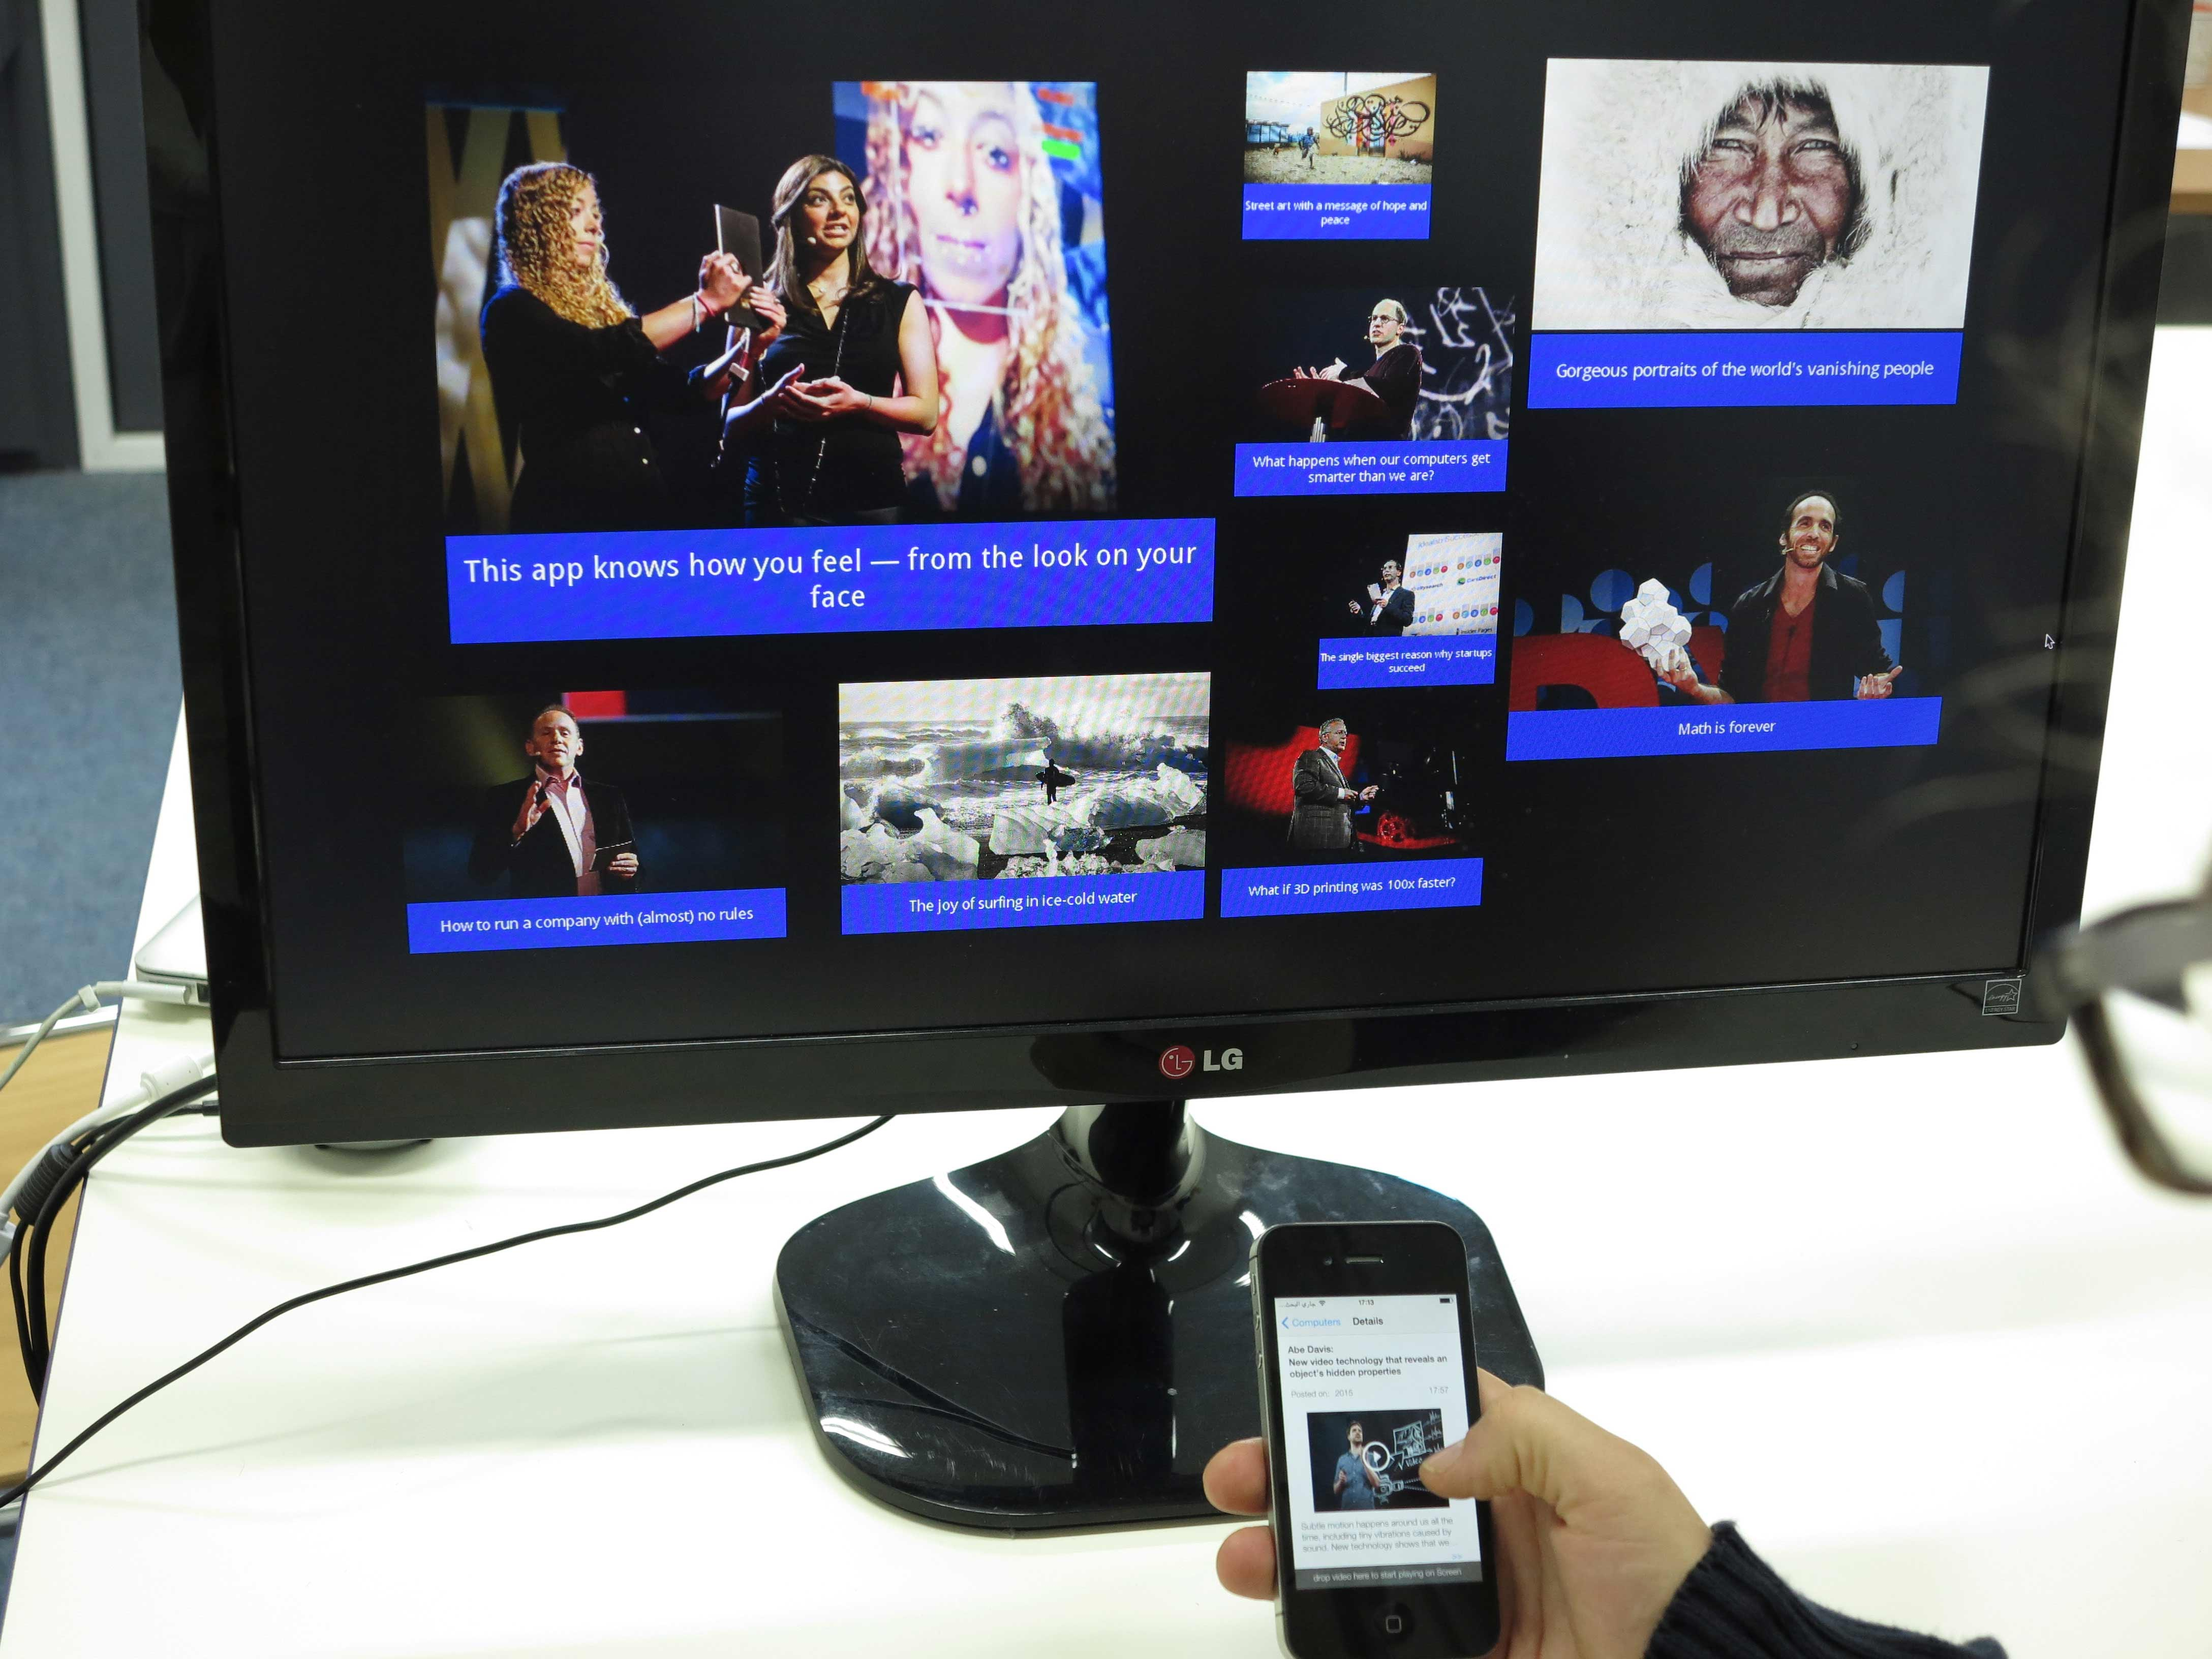
\includegraphics[width=0.75\textwidth, center, center]{figures/IMG_6806}
\caption{Participant's interaction with DiRec during the study.}
\label{fig:figure51}
\end{figure}
\subsection{Phase 2: Prototypes' Functionalities Test}
The user test was done after the participant was made familiar with the apps and
with the tasks of the study. Figures \ref{fig:figure51}, \ref{fig:figure52a},
\ref{fig:figure52b}, \ref{fig:figure52c} shows part of one of the participant's
interaction with DiRec during phase 2 of the user study. Each participant was given an iPhone mobile device with MiRec and DiRec installed, and was asked to sit across of an LD screen, which works as a display to DiRec's LD component.
Participants were asked to start with the app version of their choice to avoid
bias. After they are done with a given version, they start the tasks of the
second version. The tasks were put in place so as to have a standard set of
steps that all participants do. These steps (appendix \ref{chapter:appendB})
mainly consist of:
navigating the list of recommendations through the Home screen, viewing video details, playing
a video, rating a video, selecting a category of choice from the side menu, and
for DiRec, filtering was added to this list. By the end of each set of steps in
each app, we note that optionally users could then proceed interacting with the
apps for whichever scenarios they have in mind. Participants were informed that
this session would on average take between 15 to 20 minutes but they were also
asked to take their time or to stop the experiment at any time if they feel they
are already done and have a feel of the apps already formed. Participants were
observed during this test session, as part of the evaluation is to see how users react to the distribution aspect of the app.
Our observations of participants' interactions constitute part of our evaluation
of the results as shown later in the result section.

%%%%%%%%%%%%%%%%%%%%%%%%%%%%%%%%%%%%%%%%%%%%%%%%%%%%%%%%%%%%
\begin{figure}
    \centering
    \begin{subfigure}[b]{0.3\textwidth}
        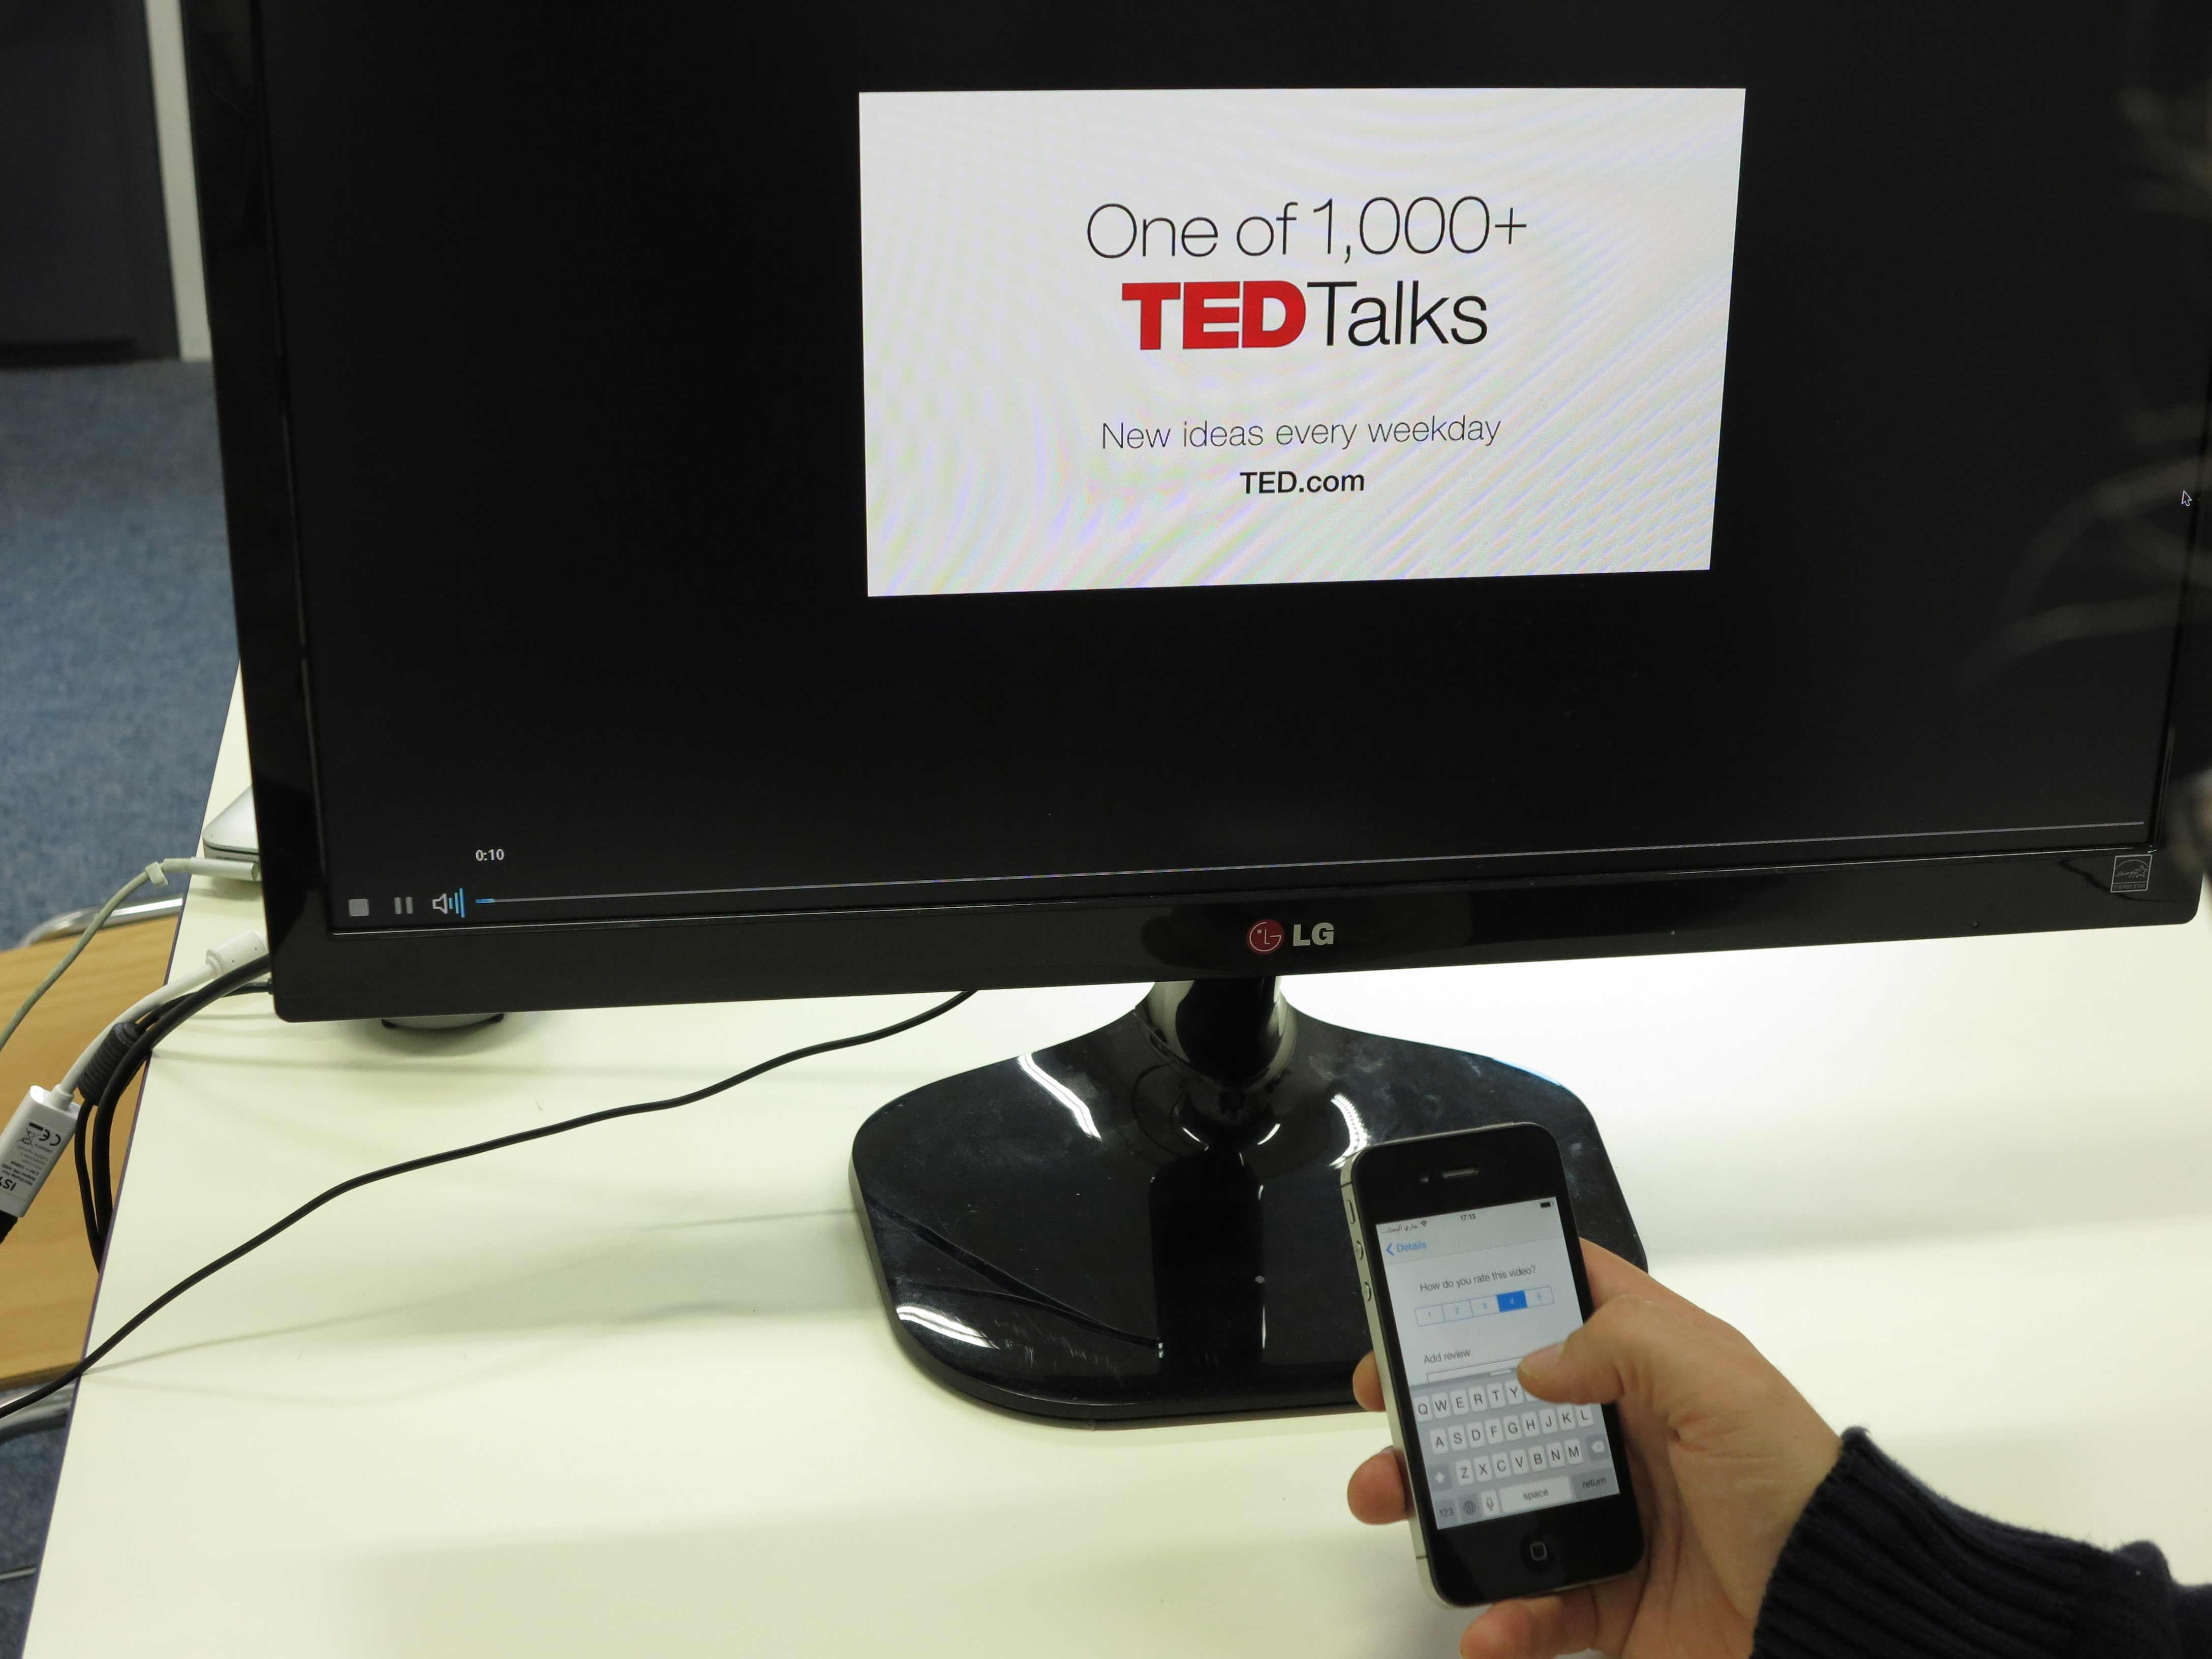
\includegraphics[width=\textwidth]{figures/IMG_6807}
        \caption{Rating and playing a video.}
        \label{fig:figure52a}
    \end{subfigure}
   
    \begin{subfigure}[b]{0.3\textwidth}
        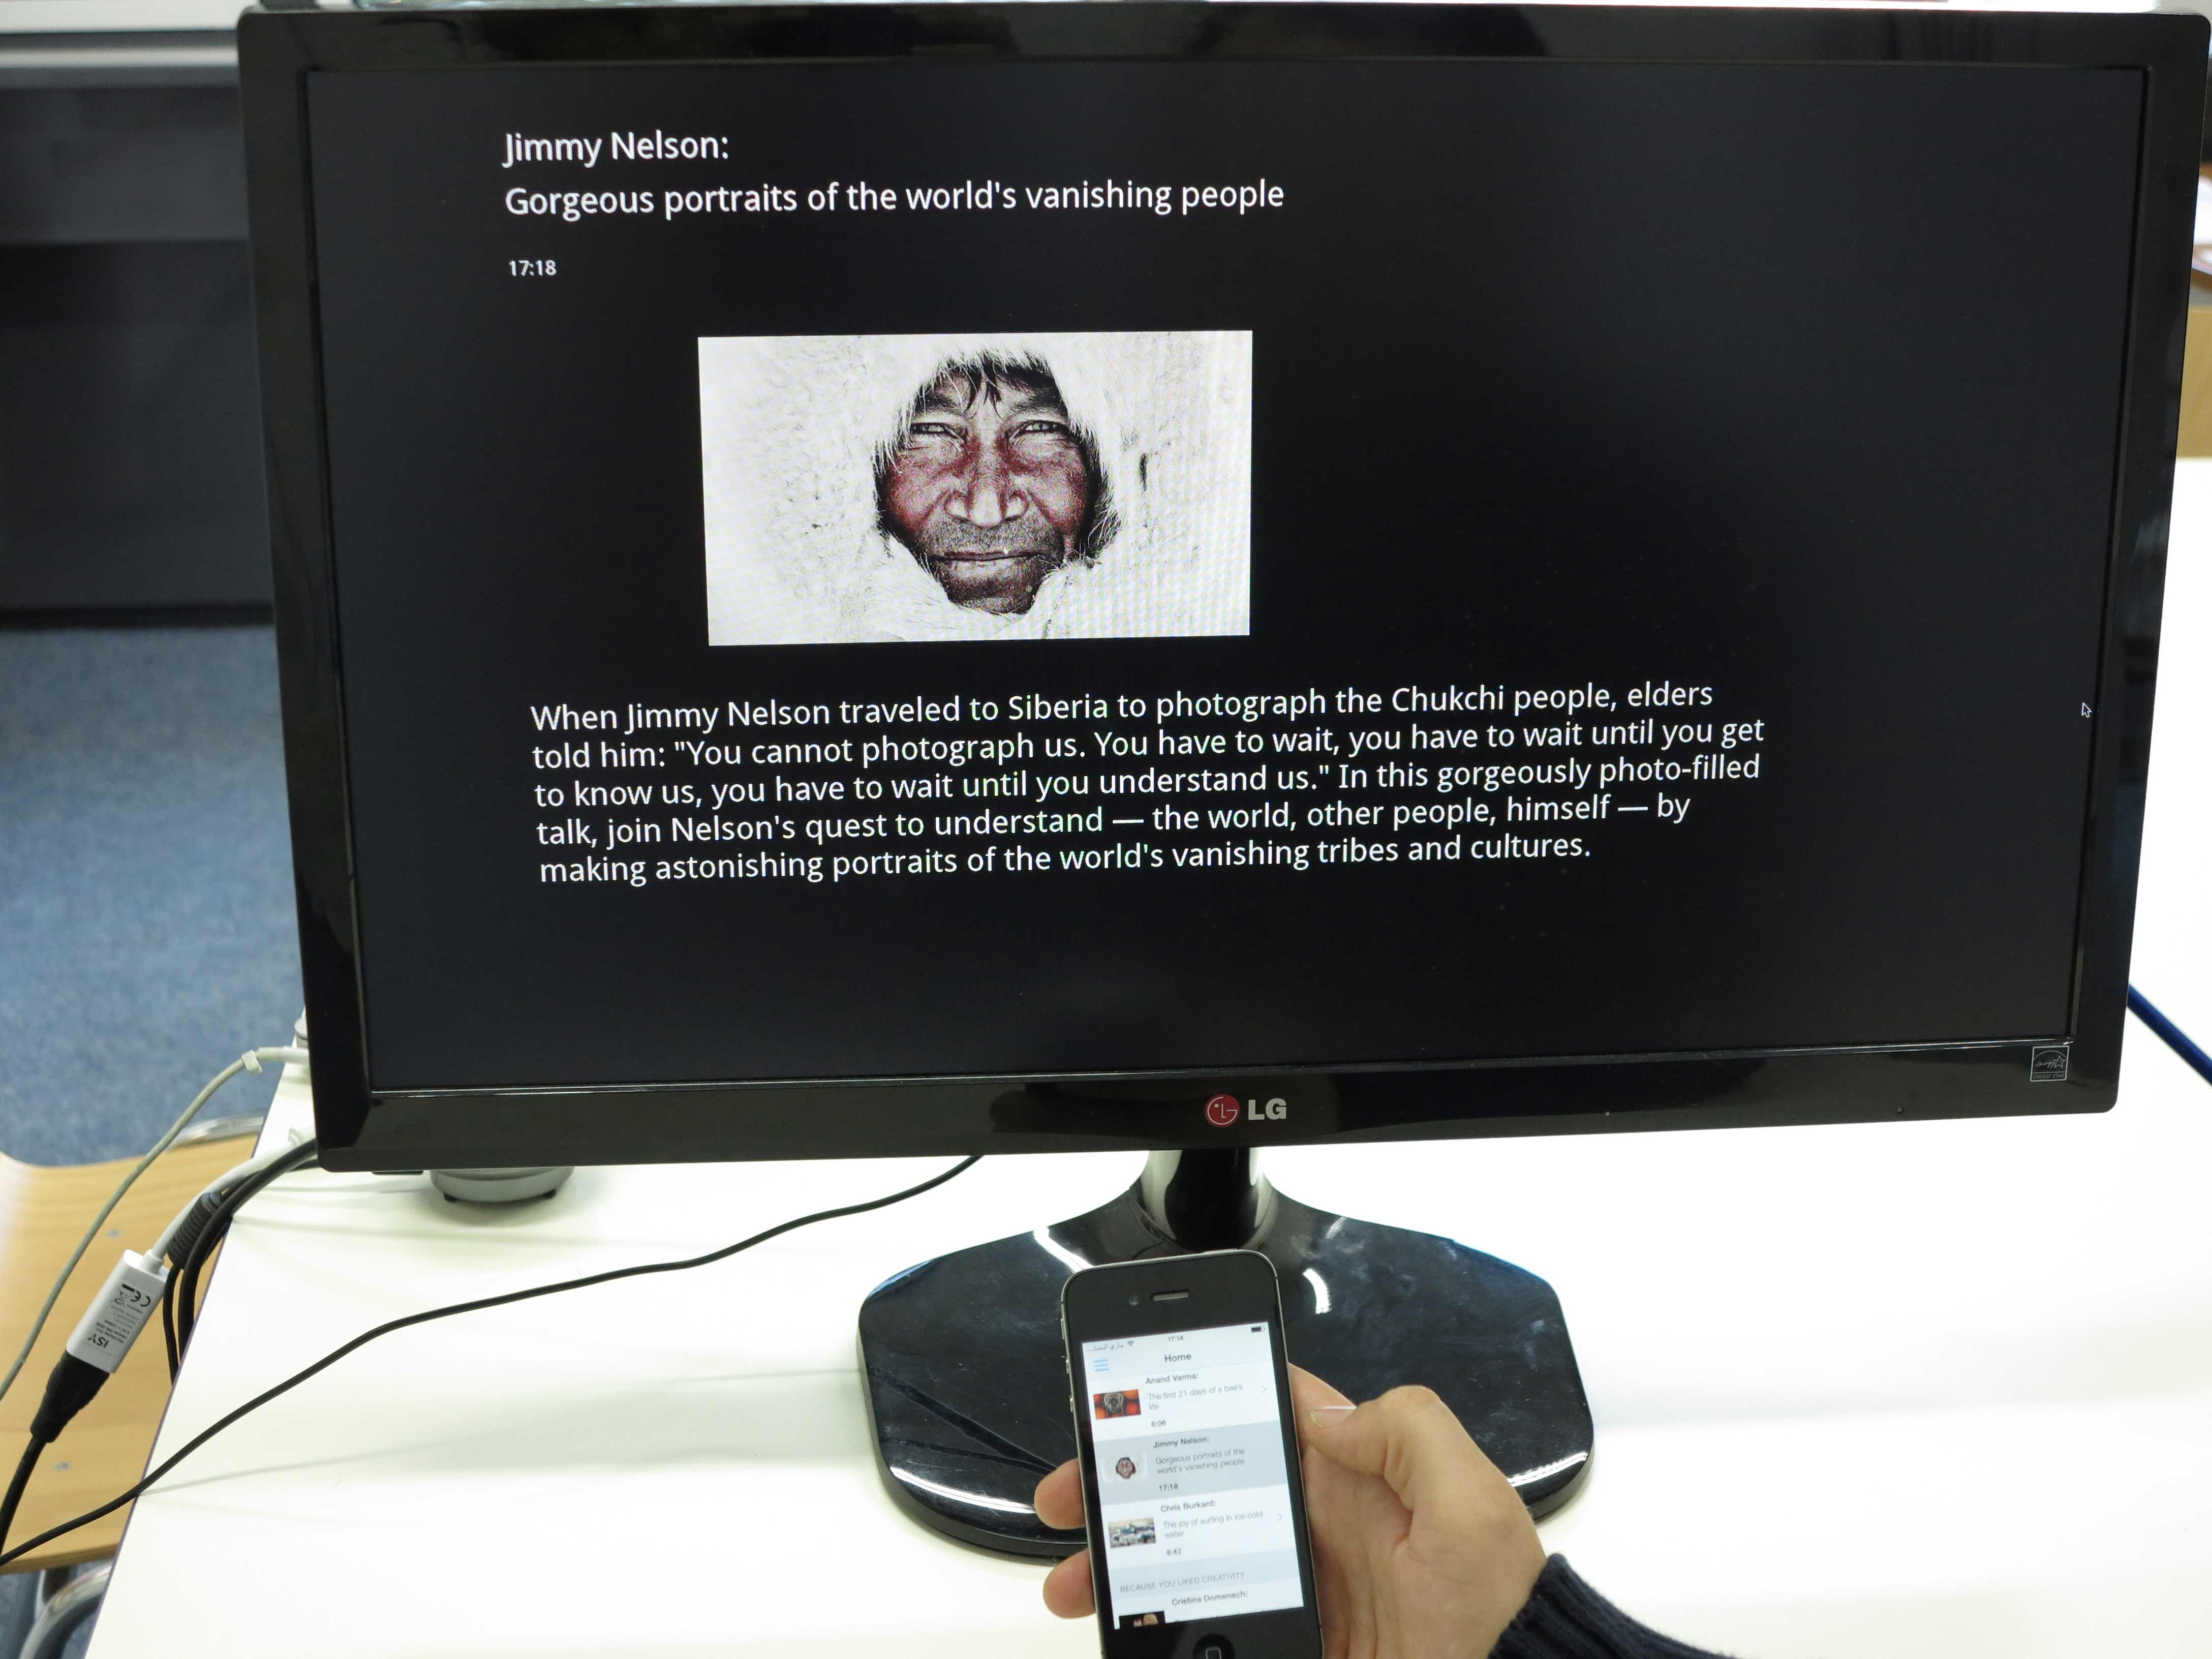
\includegraphics[width=\textwidth]{figures/IMG_6809}
        \caption{Viewing video details on DiRec}
        \label{fig:figure52b}
    \end{subfigure}
    
    \begin{subfigure}[b]{0.3\textwidth}
        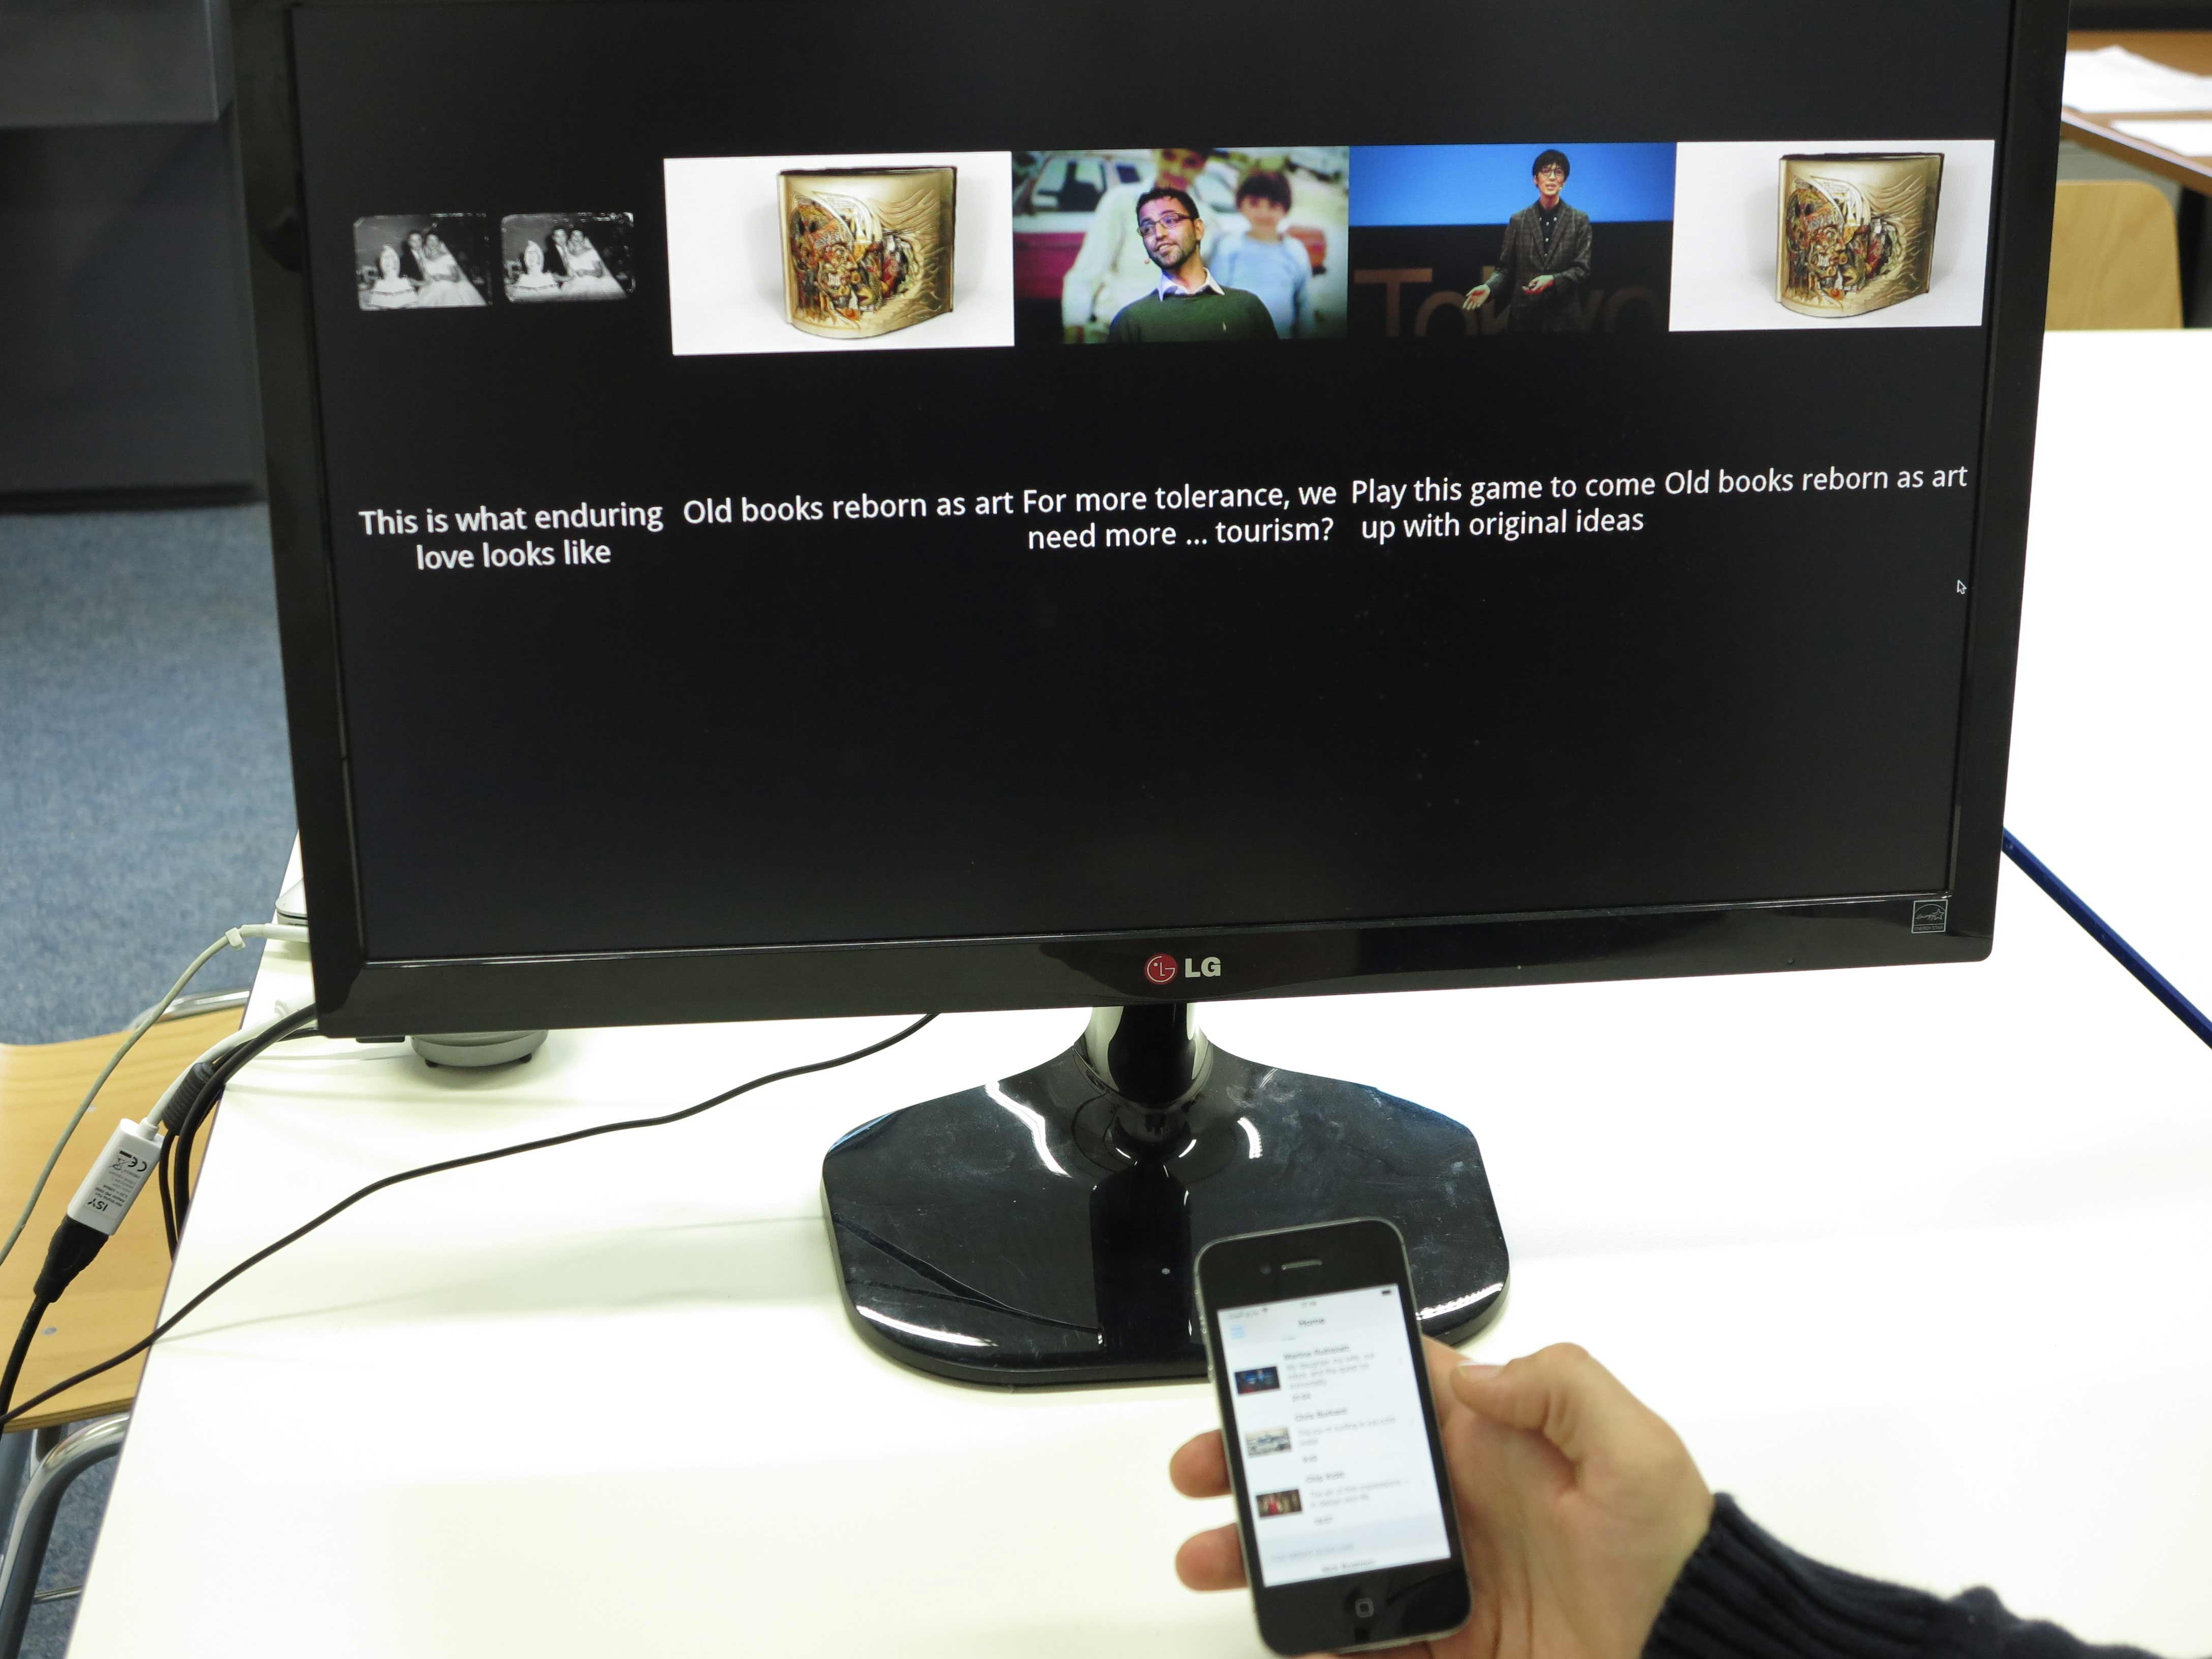
\includegraphics[width=\textwidth]{figures/IMG_6810}
        \caption{Filtering videos}
        \label{fig:figure52c}
    \end{subfigure}
   \caption{Interacting with DiRec.}\label{fig:figure52}
\end{figure}
%%%%%%%%%%%%%%%%%%%%%%%%%%%%%%%%%%%%%%%%%%%%%%%%%%%%%%%%%%%%
 
\subsection{Phase 3: Post-Experiment Survey}
For eliciting participants' feedback, we use the User Experience Questionnaire
(UEQ) suggested by Laugwitz et al.
\cite{laugwitz2008construction}. This questionnaire is designed to elicit users
direct impression through rating of a set of 26 different attributes of the
apps on a scale from 1 to 7. For the study, each participant was given 2
sheets of the UEQ test and was asked to give their ratings for each app
separately, directly after she/he is done with using the apps. She/He were also
asked to not take more than 3 to 5 minutes in each evaluation, and not to analyse her
answers, as the goal is to get her overall direct impression. Appendix \ref{chapter:appendA}
show all of the 26 aspects that users were to rate. Participants were also asked
to write down their overall feedback and comment in textual form in case they
have any. Some participants preferred to give their feedback directly to us
verbally after the study was complete. We took the change to also interview some
of the participants and ask them about what she/he liked or disliked
specifically about the apps which was valuable to our analysis. Details of our
post-experiment interviews are given in the results section.

\section{Participants Demographics}
24 participants joined our study, non of which are involved directly or
indirectly in this research.
Of the 24 participants, 19 are males and 5 are females. The age range of
participants is between 23 to 31. The majority of the participants are masters
of informatics students at TU Munich, some are researchers or developers in the
same field. We assumed that all participants have no prior knowledge in
recommender systems and explained the procedure similarly to everyone regardless
of their level of expertise.

%%%%%%%%%%%%%%%%%%%%%%%%%%%%%%%%%%%%%%%%%%%%%%%%%%%%%%%%%%%%
\begin{figure*}[t]
\centering
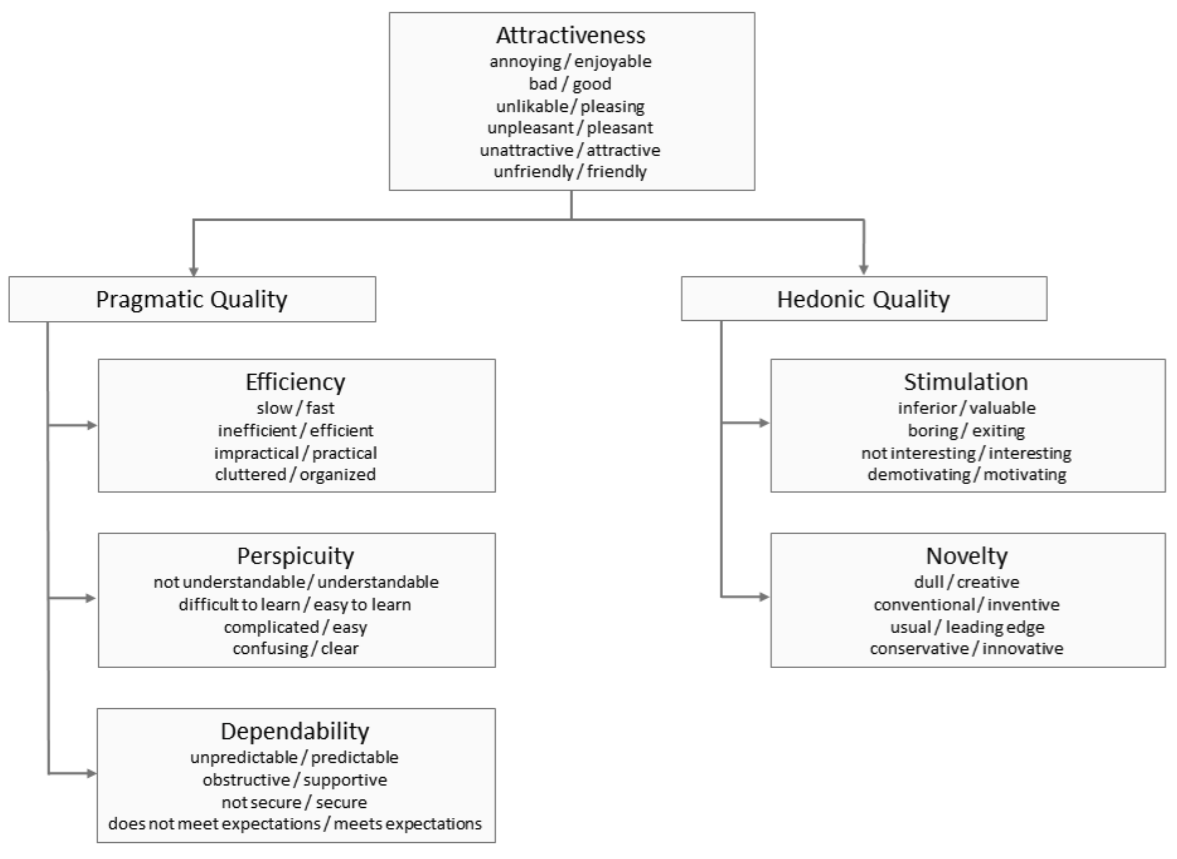
\includegraphics[width=0.7\textwidth]{figures/UEQ-scales}
\caption{User Experience Questionnaire Scale Structure. Source
\cite{UEQHandbook}.}
\label{fig:figure512}
\end{figure*}
%%%%%%%%%%%%%%%%%%%%%%%%%%%%%%%%%%%%%%%%%%%%%%%%%%%%%%%%%%%%

\section{Study Results}
\subsection{The User Experience Questionnaire}
The evaluation of participants' experiences of MiRec and DiRec is done based
on their ratings of the post User Experience Questionnaire (UEQ). The UEQ, as
explained in the UEQ handbook \cite{UEQHandbook}, consists of 6 scales with 26
items, which could be explained as follows:
\begin{itemize}
  \item \textbf{Attractiveness}: measures the overall impression or the
  likability of the product.
  \item \textbf{Perspicuity}: measures learnability and ease-of-use
  (familiarity) with the product
  \item \textbf{Efficiency}: measures the ability to perform tasks without
  exerting extra effort.
  \item \textbf{Dependability}: measures the user's control over the
  product/experience.
  \item \textbf{Stimulation}: measures how exciting and motivating the
  experience is for the user.
  \item \textbf{Novelty}: measures the level of innovation and creativity of the
  product, and the ability of the product to catch the user's interest.
\end{itemize}
These 6 scales are further categorized into 3 groups of qualities:
\textbf{\textit{Attractiveness}}, \textbf{\textit{Pragmatic
Qualities}} (Perspicuity, Efficiency, Dependability), and
\textbf{\textit{Hedonic Qualities}}(Stimulation and Novelty). Figure
\ref{fig:figure512} shows the exact items that participants rated and which
category/scale they fall under.\\
UEQ uses the Alpha Coefficient to measure the consistency of a scale i.e.
all items in a given scale  measure the aspect or quality that is meant to be
measured by this scale.
We need to consider this value in our evaluation since sometimes it is the case
that users could misinterpret a given item, or a given item could be irrelevant
to a study. Therefore, a misinterpreted item in a scale could be detected by
looking at the individual mean value per item. For example, of all items in the
scale have positive values except for a single item that has a negative value,
then it is likely that this item is misinterpreted by participants and should be
evaluated cautiously.\\
The application of the UEQ for measuring the different aspects of users
experience of a given application could be done in 2 ways. If the test involves
comparison of features or experiences of 2 versions fo the same application
(for example a new version of a given product to an older version), one could
use the \textbf{UEQ Compare of Scales Means} method, in which all of the UEQ
scales are compared for the 2 versions to show if one version is significantly different
from the other with respect to each aspect (attractiveness, perspicuity,
efficiency, etc\ldots). In a graphical representation of such comparison,
error bars are shown which indicate a 95\% confidence interval. Confidence
intervals is a measure for the accuracy of the measurements. As explained in
\cite{UEQHandbook}, since scale means would never be the same if the same
experiment was repeated a given number of times, the confidence interval of 95\%
shows where 95\% of the scales means are located. Therefore, if the error bars
(confidence intervals), of the compared products do not overlap at all, this
indicates a significant difference in the 5\% level of the measured scale.\\
The other test could be done on individual products given directly the results
of the means of the different scales. This test could show if a given
application has sufficient user experience i.e. if it meets general
expectations concerning users experience.Scales are measured between -3
(extremely bad) and +3 (extremely good). The test also provides a benchmark of
163 products to classify evaluated applications against. Results put the
evaluated applications as excellent, good, above average, bellow average,
or bad. The UEQ could also be used to make educated guesses about the possible
areas of improvement for a given evaluated application.\\
For the evaluation of our study, we apply both the comparison model between
MiRec and DiRec, as well as individual evaluations for MiRec and DiRec, with a
given comparison with benchmark studies.
\subsection{MiRec Results}
In this section we present the results of MiRec's ratings. We
examine the consistency of UEQ scales, as well as where MiRec stands in
comparison to UEQ's benchmark.
%%%%%%%%%%%%%%%%%%%%%%%%%%%%%%%%%%%%%%%%%%%%%%%%%%%%%%%%%%%%
\begin{figure}[!htbp] 
\centering
\begin{subfigure}[b]{0.45\textwidth} 
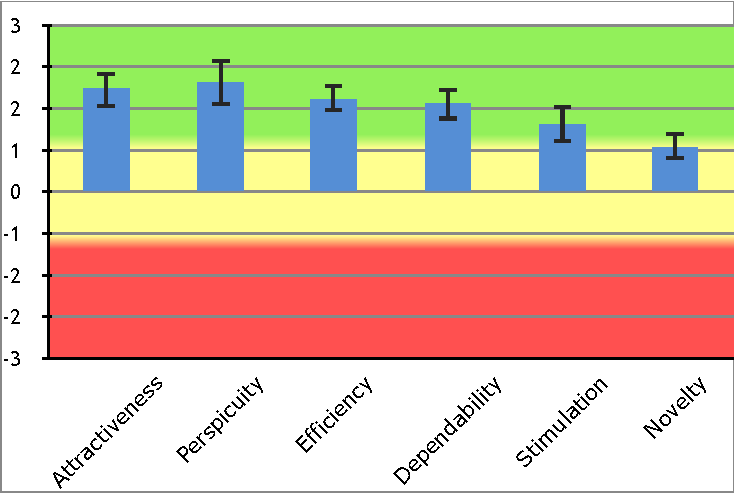
\includegraphics[width=\textwidth]{figures/mirec-results}
\caption{MiRec Scale Means.} 
\label{fig:figure54b}
\end{subfigure}
\begin{subfigure}[b]{0.45\textwidth}
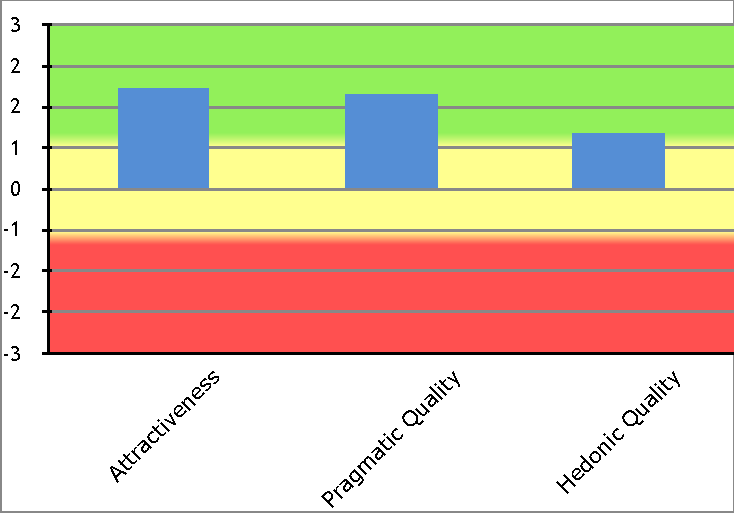
\includegraphics[width=\textwidth]{figures/mirec-results2}
\caption{MiRec Grouped Scales.}
\label{fig:figure54a}
\end{subfigure}
\caption{MiRec Scale Means.}
\label{fig:figure54}
\end{figure}
%%%%%%%%%%%%%%%%%%%%%%%%%%%%%%%%%%%%%%%%%%%%%%%%%%%%%%%%%%%%
\subsubsection{UEQ Scale Means}
UEQ's scales' means for MiRec is given in figure\ref{fig:figure54}. Figure
\ref{fig:figure54a} show the detailed scales, while figure \ref{fig:figure54b}
show the grouped scales. All of the scales show a positive evaluation (above
+0.8). As noticed, attractiveness and pragmatic qualities scores much higher
than hedonic qualities (novelty and stimulation). Nevertheless, all of the scales range in
the yellow and green sections which indicate a positive evaluation.
\subsubsection{Quality of Results: Data and Scales Consistency}
Table \ref{table:table55} shows the 5\% confidence intervals of
the scales means. All of the scales means have a relatively small confidence
interval which shows that most of the participants' opinions with respect to
the different scales were consistent, which gives us a strong reason to trust
the results.
%%%%%%%%%%%%%%%%%%%%%%%%%%%%%%%%%%%%%%%%%%%%%%%%%%%%%%%%%%%%
\begin{table}[!htbp]
\tiny 
\centering
\begin{tabular}{|l|l|l|l|l|l|l|}
\hline
\multicolumn{7}{|c|}{\textbf{Confidence intervals (p=0.05) per scale}}                                                                              \\ \hline
\textbf{Scale}          & \textbf{Mean} & \textbf{Std. Dev.} & \textbf{N} & \textbf{Confidence} & \multicolumn{2}{l|}{\textbf{Confidence interval}} \\ \hline
\textbf{Attractiveness} & 1.850         & 0.791              & 24         & 0.317               & 1.533                   & 2.167                   \\ \hline
\textbf{Perspicuity}    & 1.950         & 1.026              & 24         & 0.410               & 1.540                   & 2.360                   \\ \hline
\textbf{Efficiency}     & 1.675         & 0.624              & 24         & 0.250               & 1.425                   & 1.925                   \\ \hline
\textbf{Dependability}  & 1.575         & 0.736              & 24         & 0.295               & 1.280                   & 1.870                   \\ \hline
\textbf{Stimulation}    & 1.225         & 0.854              & 24         & 0.341               & 0.884                   & 1.566                   \\ \hline
\textbf{Novelty}        & 0.825         & 0.635              & 24         & 0.254               & 0.571                   & 1.079                   \\ \hline
\end{tabular}
\caption{Confidence Interval MiRec.}
\label{table:table55}
\end{table}
%%%%%%%%%%%%%%%%%%%%%%%%%%%%%%%%%%%%%%%%%%%%%%%%%%%%%%%%%%%%
\\
Figure \ref{fig:figure56} shows the means values per item, which is an indicator
to the consistency of how users interpreted the different items in a given
scale. As shown, different items in a given scale are shown in the same color.
Since all items of all scales have positive means, this could indicate that
there were not misinterpreted items in any scale.\\

UEQ provides a way to detect inconsistent data in a given scale. Since not all
of the participant would give correct or serious ratings, we needed a way to
know if there are any discrepancies in the data. Our results show 2 out of
the 24 participants who gave inconsistent ratings to 3 of the scales. 1
participant gave 2 inconsistent scales ratings, 9 participants gave 1
inconsistent scale ratings. This on average means that the data was sufficiently
consistent.
%%%%%%%%%%%%%%%%%%%%%%%%%%%%%%%%%%%%%%%%%%%%%%%%%%%%%%%%%%%%
\begin{figure*}[!htbp]
\centering
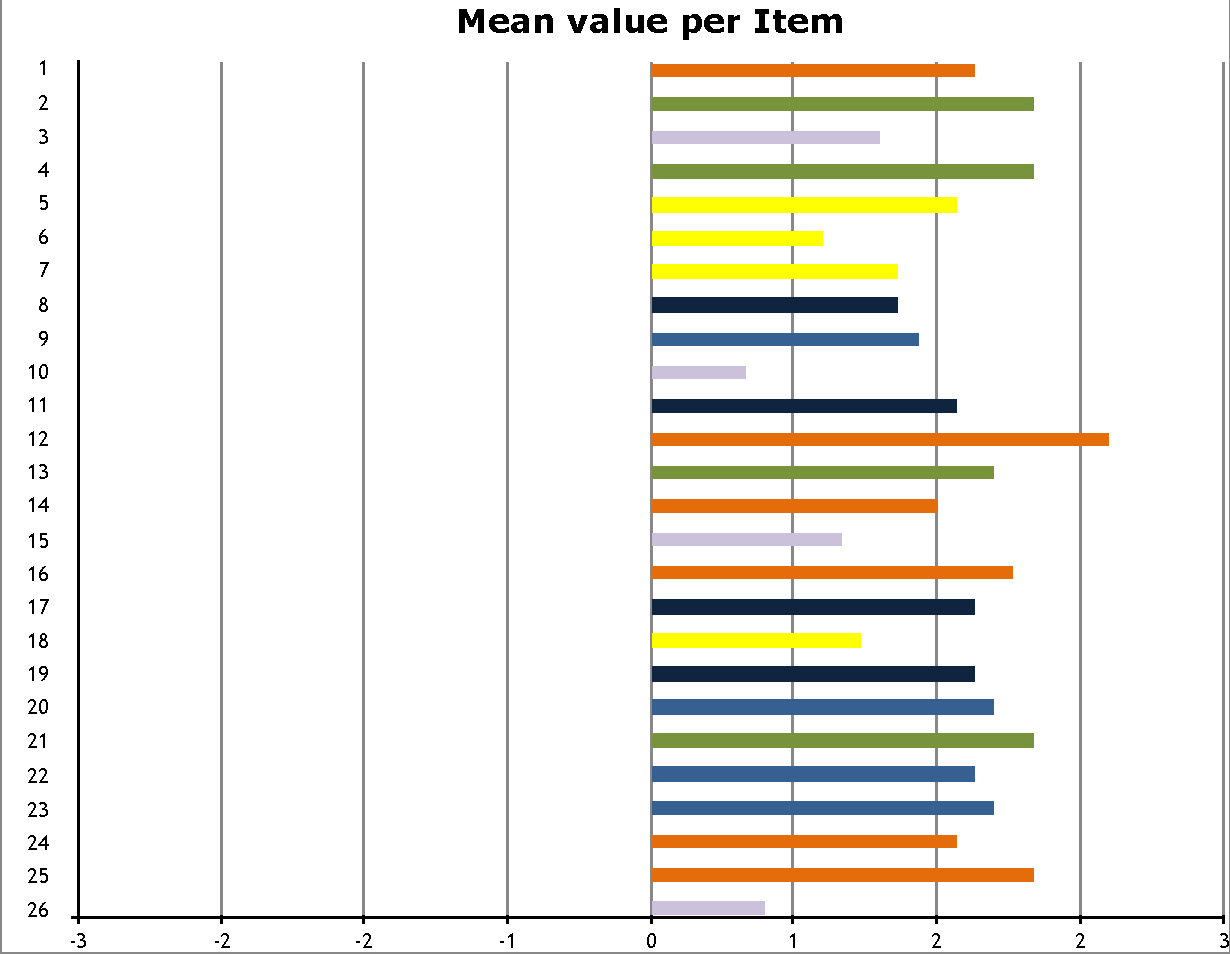
\includegraphics[width=0.7\textwidth]{figures/mirec-results3}
\caption{MiRec Mean Value Per Item.}
\label{fig:figure56}
\end{figure*}
%%%%%%%%%%%%%%%%%%%%%%%%%%%%%%%%%%%%%%%%%%%%%%%%%%%%%%%%%%%%
\subsubsection{Comparison of MiRec to UEQ Benchmark}
Figure \ref{fig:figure57} and table \ref{table:table54} show the results of
comparing MiRec's scales means to UEQ's benchmark. As it is shown, MiRec's
attractiveness measure in the the range of 10\% of best results (excellent).
With respect to dependability, MiRec is better than 75\% of the results, and
worse than 10\% of the results (good). When it comes to stimulation and novelty,
MiRec is better than 50\% of the results, while worse than 25\% of the results
(above average). 
%%%%%%%%%%%%%%%%%%%%%%%%%%%%%%%%%%%%%%%%%%%%%%%%%%%%%%%%%%%%
\begin{table}[!htbp]
\tiny
\centering
\begin{tabular}{|l|l|l|l|}
\hline
\textbf{Scale}          & \textbf{Mean} & \textbf{Comparison to benchmark} & \textbf{Interpretation}                       \\ \hline
\textbf{Attractiveness} & 1.850         & Excellent                         & In the range of the 10\% best results         \\ \hline
\textbf{Perspicuity}    & 1.950         & Excellent                         & In the range of the 10\% best results         \\ \hline
\textbf{Efficiency}     & 1.675         & Excellent                         & In the range of the 10\% best results         \\ \hline
\textbf{Dependability}  & 1.575         & Good                              & 10\% of results better, 75\% of results worse \\ \hline
\textbf{Stimulation}    & 1.225         & Above Average                     & 25\% of results better, 50\% of results worse \\ \hline
\textbf{Novelty}        & 0.825         & Above Average                     & 25\% of results better, 50\% of results worse \\ \hline
\end{tabular}
\caption{Comparison of MiRec to UEQ Benchmark}
\label{table:table54}
\end{table}
%%%%%%%%%%%%%%%%%%%%%%%%%%%%%%%%%%%%%%%%%%%%%%%%%%%%%%%%%%%%
%%%%%%%%%%%%%%%%%%%%%%%%%%%%%%%%%%%%%%%%%%%%%%%%%%%%%%%%%%%%
\begin{figure*}[!htbp]
\centering
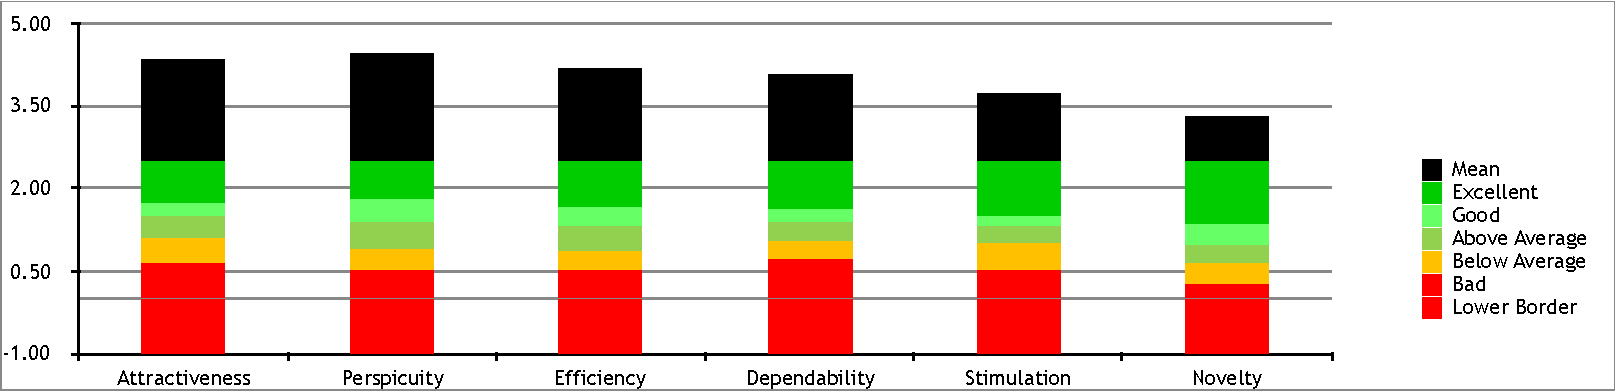
\includegraphics[width=0.9\textwidth]{figures/mirec-benchmark}
\caption{MiRec Comparison to Benchmark Studies.}
\label{fig:figure57}
\end{figure*}
%%%%%%%%%%%%%%%%%%%%%%%%%%%%%%%%%%%%%%%%%%%%%%%%%%%%%%%%%%%%


\subsection{DiRec Results}
Similarly to the previous section, in this section, we are going to present the
results for DiRec through the UEQ scales means. The results quality will also be
investigated. And lastly, a comparison of DiRec with UEQ benchmark will be
provided.
%%%%%%%%%%%%%%%%%%%%%%%%%%%%%%%%%%%%%%%%%%%%%%%%%%%%%%%%%%%%
\begin{figure}[!htbp]
\centering
\begin{subfigure}[b]{0.45\textwidth}
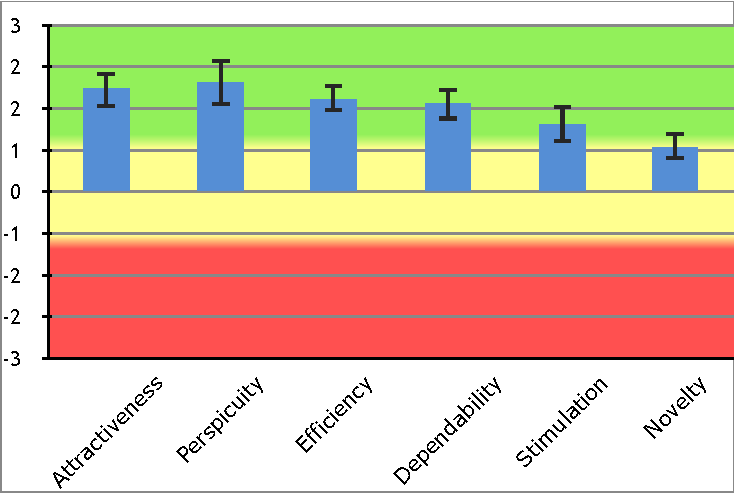
\includegraphics[width=\textwidth]{figures/direc-results}
\caption{Scale Means.}
\label{fig:figure516a}
\end{subfigure}
\begin{subfigure}[b]{0.45\textwidth}
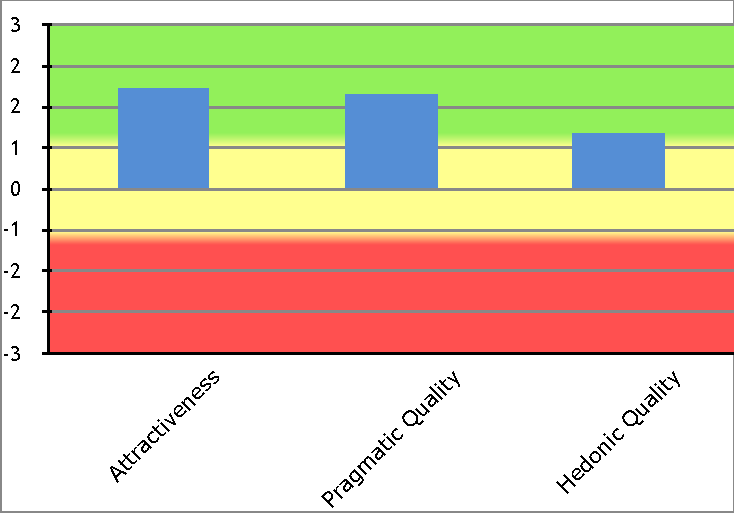
\includegraphics[width=\textwidth]{figures/direc-results2}
\caption{Grouped Scale Means.}
\label{fig:figure516b}
\end{subfigure}
\caption{DiRec Scale Means.}
\label{fig:figure516}
\end{figure}
%%%%%%%%%%%%%%%%%%%%%%%%%%%%%%%%%%%%%%%%%%%%%%%%%%%%%%%%%%%%
\subsubsection{UEQ Scale Means}
Figure \ref{fig:figure516} show DiRec's UEQ scale means. The 6 UEQ scales are
given in figure \ref{fig:figure516a} while the grouped scales are given in
figure \ref{fig:figure516b}. Similar to MiRec, DiRec scale means show a
positive evaluation (> +0.8). Attractiveness, pragmatic qualities, and hedonic qualities,
all fall in the green (best) and yellow (good) sections. Higher ratings are
given to attractiveness and pragmatic qualities than hedonic qualities. However,
hedonic qualities still get a positive evaluation.


\subsubsection{Quality of Results: Data and Scales Consistency}
To test the data and scales dependability and consistency, we also look at
the confidence intervals of the scale means. The 5\% confidence intervals of
DiRec is shown in table \ref{table:table57}. The intervals for all scales are
also relatively small, which means that participants opinions with respect to
the different scales were also consistent for DiRec.
%%%%%%%%%%%%%%%%%%%%%%%%%%%%%%%%%%%%%%%%%%%%%%%%%%%%%%%%%%%%
\begin{table}[!htbp]
\tiny
\centering
\begin{tabular}{|l|l|l|l|l|l|l|}
\hline
\multicolumn{7}{|c|}{\textbf{Confidence intervals (p=0.05) per scale}}         
\\\hline \textbf{Scale}          & \textbf{Mean} & \textbf{Std. Dev.} &
\textbf{N} &\textbf{Confidence} & \multicolumn{2}{l|}{\textbf{Confidence interval}} \\\hline \textbf{Attractiveness} & 1.850         & 0.791              & 24         &0.317               & 1.533                   & 2.167                  \\\hline 
\textbf{Perspicuity}    & 1.950         & 1.026              & 24         &
0.410               & 1.540                   & 2.360                 \\\hline
\textbf{Efficiency}     & 1.675         & 0.624              & 24         &
0.250               & 1.425                   & 1.925                 \\\hline
\textbf{Dependability}  & 1.575         & 0.736              & 24         &
0.295               & 1.280                   & 1.870                 \\\hline
\textbf{Stimulation}    & 1.225         & 0.854              & 24         &
0.341               & 0.884                   & 1.566                 \\\hline
\textbf{Novelty}        & 0.825         & 0.635              & 24         &
0.254               & 0.571                   & 1.079  \\\hline
\end{tabular}
\caption{DiRec Confidence Intervals.}
\label{table:table57}
\end{table}
%%%%%%%%%%%%%%%%%%%%%%%%%%%%%%%%%%%%%%%%%%%%%%%%%%%%%%%%%%%%
For further investigation of the consistency of individual scales, we look at
the means values per item per scale, which is shown in figure
\ref{fig:figure510}. The consistency of the items' ratings is evident
as all items of different scales have positive means. This give us strong
reasons to trust the data of DiRec and believe that misinterpretations were
minimum.\\
Moreover, we use UEQ's method of tacking data discrepancies caused by
inaccurate ratings. of the 24 participants, 3 participants provide inaccurate
ratings for 3 different scales, and 3 others provide inaccurate ratings for 2
scales. The remaining ratings fall in the trusted range. This also shows that
the results are mostly sufficiently reliable.
%%%%%%%%%%%%%%%%%%%%%%%%%%%%%%%%%%%%%%%%%%%%%%%%%%%%%%%%%%%%
\begin{figure*}[!htbp]
\centering
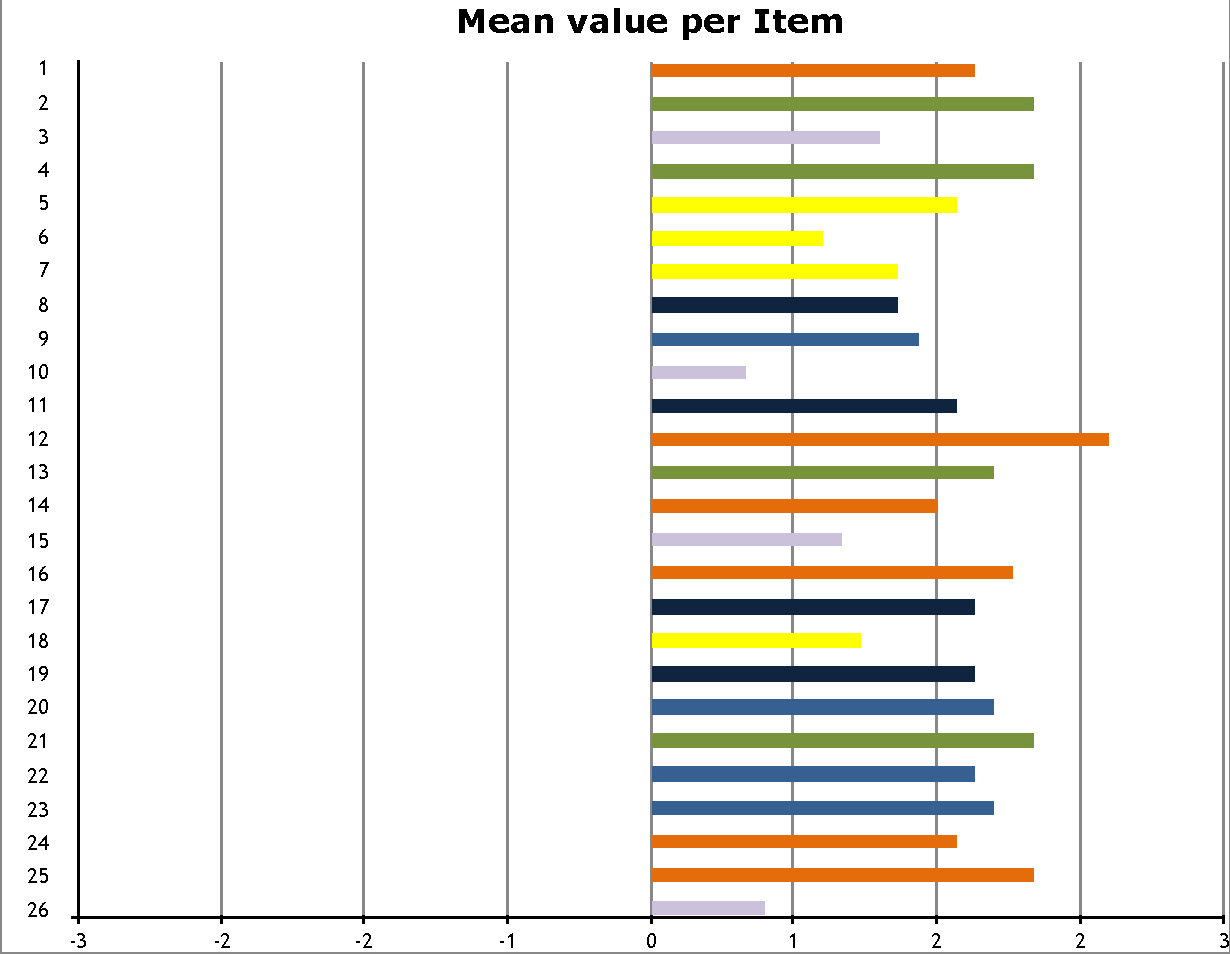
\includegraphics[width=0.7\textwidth]{figures/direc-results3}
\caption{DiRec Mean Value Per Item.}
\label{fig:figure510}
\end{figure*}
%%%%%%%%%%%%%%%%%%%%%%%%%%%%%%%%%%%%%%%%%%%%%%%%%%%%%%%%%%%%
\subsubsection{Comparison of DiRec to UEQ Benchmark}
The results of comparing the results of DiRec scale means to UEQ's benchmark is
shown in figure \ref{fig:figure511} and table \ref{table:table56}. DiRec's
attractiveness, perspicuity, and efficiency measure in the the range of the 10\%
best results (excellent). While dependability scored 75\% better than other
results, and 10\% worse (good). For stimulation and novelty, the scores were
above average, with 50\% of the results wore than DiRec, and 25\% of the results
better than DiRec. This is in general a good indicator to where DiRec stands in
comparison to other studies evaluated using the same method.

%%%%%%%%%%%%%%%%%%%%%%%%%%%%%%%%%%%%%%%%%%%%%%%%%%%%%%%%%%%%
\begin{table}[!htbp]
\tiny
\centering
\begin{tabular}{|l|l|l|l|}
\hline
\textbf{Scale}          & \textbf{Mean} & \textbf{Comparison to benchmark} & \textbf{Interpretation}                       \\ \hline
\textbf{Attractiveness} & 1.850         & Excellent                         & In the range of the 10\% best results         \\ \hline
\textbf{Perspicuity}    & 1.950         & Excellent                         & In the range of the 10\% best results         \\ \hline
\textbf{Efficiency}     & 1.675         & Excellent                         & In the range of the 10\% best results         \\ \hline
\textbf{Dependability}  & 1.575         & Good                              & 10\% of results better, 75\% of results worse \\ \hline
\textbf{Stimulation}    & 1.225         & Above Average                     & 25\% of results better, 50\% of results worse \\ \hline
\textbf{Novelty}        & 0.825         & Above Average                     & 25\% of results better, 50\% of results worse \\ \hline
\end{tabular}
\caption{DiRec Comparison to Benchmark Studies.}
\label{table:table56}
\end{table}
%%%%%%%%%%%%%%%%%%%%%%%%%%%%%%%%%%%%%%%%%%%%%%%%%%%%%%%%%%%%
%%%%%%%%%%%%%%%%%%%%%%%%%%%%%%%%%%%%%%%%%%%%%%%%%%%%%%%%%%%%
\begin{figure*}[!htbp]
\centering
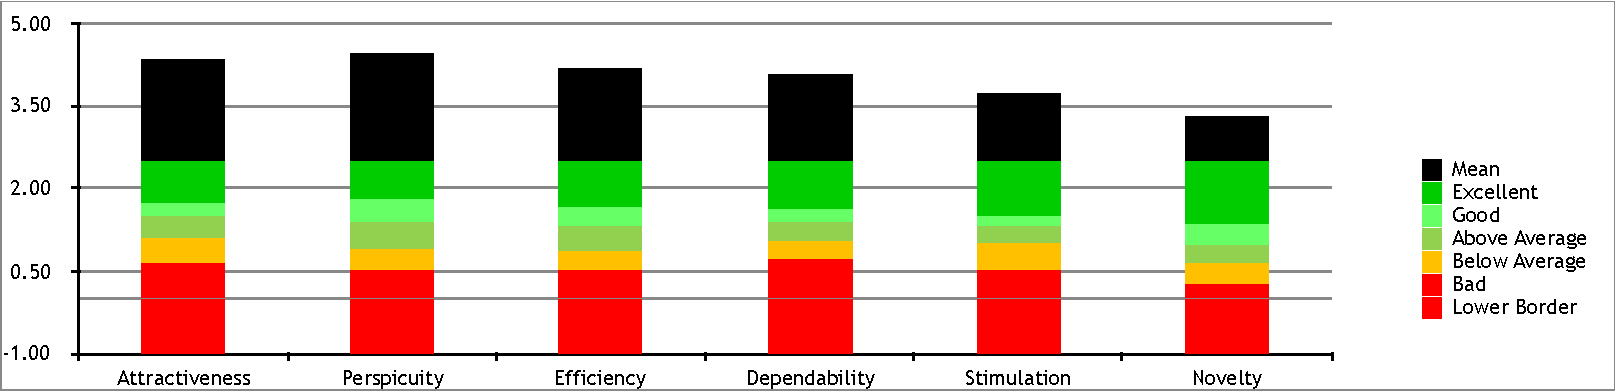
\includegraphics[width=0.9\textwidth]{figures/direc-benchmark}
\caption{Comparison of DiRec to Benchmark Studies.}
\label{fig:figure511}
\end{figure*} 
%%%%%%%%%%%%%%%%%%%%%%%%%%%%%%%%%%%%%%%%%%%%%%%%%%%%%%%%%%%%
\subsection{MiRec and DiRec Compared Using UEQ Scales}
UEQ provides an automated way to compare the results of 2 products with respect
to scales means. Figure \ref{fig:figure53} show the result of this comparison
for MiRec(left side, blue) and Direc (right side, red). With respect to
attractiveness, stimulation, and novelty, DiRec scores higher than MiRec. For
efficiency and dependability, they measure almost similarly with MiRec scoring
slightly better than DiRec. MiRec, however, scores much higher than DiRec when
it comes to the perspicuity scale.
%%%%%%%%%%%%%%%%%%%%%%%%%%%%%%%%%%%%%%%%%%%%%%%%%%%%%%%%%%%%
\begin{figure*}[!htbp]
\centering
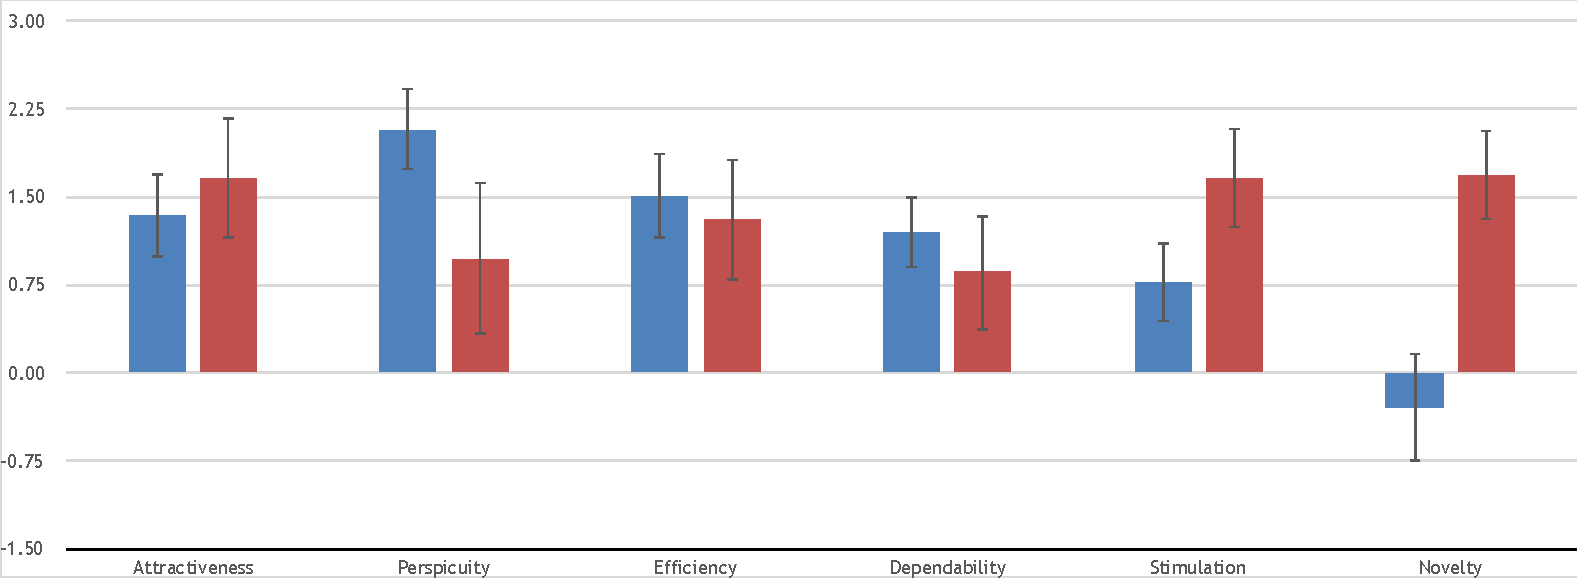
\includegraphics[width=0.95\textwidth]{figures/compare}
\caption{Comparison of Scale Means in MiRec and DiRec.}
\label{fig:figure53}
\end{figure*}
%%%%%%%%%%%%%%%%%%%%%%%%%%%%%%%%%%%%%%%%%%%%%%%%%%%%%%%%%%%%

UEQ further uses The T-Test to check if the scale means of two measured
applications differ significantly. As a default, an Alpha-Level 0.05 is used.
Table \ref{table:table53} show the results of the T-Test. As shown, MiRec and
DiRec differ significantly with respect to 3 of the scales: Perspicuity,
Stimulation, and Novelty. As mentioned earlier, DiRec scores significantly lower
than MiRec when it comes to the perspicuity scale, however, it scores
significantly higher when it comes to stimulation, and even higher when it
comes to novelty. Moreover, according to the T-Test, the difference between
MiRec and DiRec in attractiveness, efficiency, and dependability is not a
significant difference.

%%%%%%%%%%%%%%%%%%%%%%%%%%%%%%%%%%%%%%%%%%%%%%%%%%%%%%%%%%%%
\begin{table}[!htbp]
\centering
\tiny
\begin{tabular}{|l|l|l|}
\hline
\multicolumn{1}{|r|}{Alpha Level:} & 0.05   &                                                         \\ \hline
                                   &        &                                                         \\ \hline
\textbf{Attractiveness}            & 0.1827 & No Significant Difference       \\ \hline
\textbf{Perspicuity}               & 0.0092 & \textbf{Significant Difference} \\ \hline
\textbf{Efficiency}                & 0.7431 & No Significant Difference       \\ \hline
\textbf{Dependability}             & 0.1852 & No Significant Difference       \\ \hline
\textbf{Stimulation}               & 0.0007 & \textbf{Significant Difference} \\ \hline
\textbf{Novelty}                   & 0.0000 & \textbf{Significant Difference} \\ \hline
\end{tabular}
\caption{T-Test with Alpha Level 0.05.}
\label{table:table53}
\end{table} 

\subsection{Discussion}
In the light of the stated individual results of MiRec and DiRec, as well as the
comparison of both applications using the results of the UEQ, the following
interpretations could be made:
\subsubsection{UI Distribution aids the Stimulation and Novelty of Recommendation
Applications, hence, enriches the user's experience.} The high stimulation and
novelty ratings DiRec scored, as well as differing significantly in this aspect
from the non-distributed version MiRec, can help draw the conclusion that UI
distribution could lead to an enriching user experience from this aspect.
DiRec as a DUI has excited and motivated the user (Stimulation), as well as,
shown to be more innovative, creative and interesting (novelty) than its non
distributed counter-part.
 
\subsubsection{UI Distribution does not hinder the efficiency or limit the span
of the user's control of recommendation applications.} Despite the fact that
efficiency and dependability measures did not score higher in the distributed
solution than than the non-distributed one, they still hold a positive
evaluation that show no significant difference than the non-distributed UI
solution. This would be used to show that the user could perform tasks as
efficiently with a DUI as with a non DUI solution, with no need for extra time
or effort. It would also mean that UI distribution does not lessen or affect the
user's control of the interaction with DUI application as shown with the good
dependability measures. This also leaves a room for possible improvement in
these aspects.

\subsubsection{UI Distribution results in more attractive recommendation applications.} DiRec's good ratings of the attractiveness scale, and despite
the non significant increase it has over the non distributed version, shows that
users found the UI distribution idea generally likable and agreeable. The good
levels attractiveness MiRec scored would also mean that user still like a
non-distributed version of a recommendation application. Despite not showing in
the measurement of the scale means of the UEQ, interviewing and observing the
user study participants have shown general inclination towards liking the DUI
version better than the non-DUI version. More than 70\% of participants we
interviewed after the study mentioned that DiRec left a more agreeable
impression than MiRec, which was also shown by observing the user's interaction
with the application.

\subsubsection{UI Distribution might affect the learnability and ease-of-use of recommendation applications.}
DiRec's score was in the good range when it comes to the benchmark of UEQ, which
shows learnability, ease of use, and clarity of the application are not on a low
scale. However, the comparison with MiRec showed a significant difference. This
shows that UI distribution could affect how easy and clear it is to use,
understand, and learn a recommendation application. A few number of participants
have mentioned that they were confused by DiRec. When asked to elaborate the
soure of their confusion, most of them noted that it could be that they did not
get enough time to familiarize with the application. This leads us to believe
that there further investigation is needed to pinpoint the actual causes of the
lower ratings in this aspect to know whether it could be due to insufficient
explanation and demonstration of the study procedure, or due to other reasons.
\subsection{Participants' Suggestions}
Most participants were interviewed to give us feedback about their experience
with the systems after the study and ratings were complete. Since most
participants had no prior knowledge of what exactly we were after in our study,
we did not want to influence the participants' experience, we gave further
explanation of what we are trying to test with the user study in this phase. We
present here some of the participant's comments and suggestions concerning their
experiences.
\subsubsection{Dual Display}
The overall feedback of most participants was that they find the idea of being
able to have a video recommender application in which one control through the
phone, while being able to watch videos over a larger display, was found highly
agreeable. Some comments were: \textit{``I find the app interesting. I like to
have that for example with Whatsapp to enable me to watch videos on a bigger screen or on my laptop.''}\\
Another participant added: \textit{``I use at least 2 or 3 devices at home and
would definitely like an app that would enable me to choose one or the other, specially with watching videos. It
would be nice to have.''}  
\subsubsection{Input Redirection}
Being able to have control over the screen app in DiRec was pinpointed by a
number of participants: \textit{``Somehow I was expecting the screen app to be
the main app and the phone app to work as a remote control. I still would like to be able to
enter input to the [screen] app through the phone.''}\\
Another participant suggested having full control over video playing on the
screen app through the phone app: \textit{``A progress bar and video controllers
of the currently playing videos should be available in [DiRec]. The [phone] app should work as a remote
control.''}
\subsubsection{Filtering}
The filtering in DiRec feature was praised by most participants. One participant
particularly mentioned: \textit{``The filtering feature is nice to have. I think
I have not seen it in similar application like Chrome Cast. I would suggest to also be able to save this as
a bookmark or history so I would go back to it.''}
\subsubsection{The Use of Gestures}
In DiRec, we depended mainly on swiping and panning gestures to perform tasks.
Some the participants comments about the use of gestures: \textit{``Having to
swiping down to play the video was not very intuitive. If it was not demoed earlier, I wouldn't know that this is how I am supposed to play the
video. Swiping left and right for filtering and details was more clear.''}\\
Another participant mentioned a similar comment: \textit{``Swipe down for
playing might not be very intuitive for inexperienced users''.}
\subsubsection{Rating}
Rating a video while watching is a feature that we were interested to
know if participants found interesting or confusing. Most participants
mentioned that it was a good feature to have, but with also the
possibility to skip it. One participants commented:\textit{``Being asked to rate the video after each app in MiRec was
annoying. Preferably, I liked to be able to do the rating while watching in
[DiRec], or to be able to skip it.''}\\

%%%%%%%%%%%%%%%%%%%%%%%%%%%%%%%%%%%%%%%%%%%%%%%%%%%%%%%%%%%%
%%%%%%%%%%%%%%%%%%%%%%%%%%%%%%%%%%%%%%%%%%%%%%%%%%%%%%%%%%%%
% \begin{table}[!htbp]
% \tiny
% \centering
% \begin{tabular}{|l|l|l|l|l|l|l|}
% \hline
% \multicolumn{1}{|c|}{\multirow{2}{*}{\textbf{Scale}}} & \multicolumn{6}{c|}{\textbf{MiRec Dataset}}                                                                         \\ \cline{2-7} 
% \multicolumn{1}{|c|}{}                                & \textbf{Mean} & \textbf{STD} & \textbf{N} & \textbf{Confidence} & \multicolumn{2}{l|}{\textbf{Confidence Interval}} \\ \hline
% \textbf{Attractiveness}                               & 1.34          & 0.91         & 25         & 0.36                & 0.98                     & 1.70                   \\ \hline
% \textbf{Perspicuity}                                  & 2.08          & 0.88         & 25         & 0.35                & 1.73                     & 2.43                   \\ \hline
% \textbf{Efficiency}                                   & 1.51          & 0.91         & 25         & 0.36                & 1.15                     & 1.87                   \\ \hline
% \textbf{Dependability}                                & 1.20          & 0.76         & 25         & 0.30                & 0.90                     & 1.50                   \\ \hline
% \textbf{Stimulation}                                  & 0.78          & 0.86         & 25         & 0.34                & 0.44                     & 1.12                   \\ \hline
% \textbf{Novelty}                                      & -0.29         & 1.17         & 25         & 0.46                & -0.75                    & 0.17                   \\ \hline
% \end{tabular}
% \caption{MiRec.}
% \label{table:table51}
% \end{table}
%%%%%%%%%%%%%%%%%%%%%%%%%%%%%%%%%%%%%%%%%%%%%%%%%%%%%%%%%%%%

%%%%%%%%%%%%%%%%%%%%%%%%%%%%%%%%%%%%%%%%%%%%%%%%%%%%%%%%%%%%
% \begin{table}[!htbp]
% \tiny
% \centering  
% \begin{tabular}{|l|l|l|l|l|l|l|}
% \hline
% \multicolumn{1}{|c|}{\multirow{2}{*}{\textbf{Scale}}} & \multicolumn{6}{c|}{\textbf{DiRec Dataset}}                                                                         \\ \cline{2-7} 
% \multicolumn{1}{|c|}{}                                & \textbf{Mean} & \textbf{STD} & \textbf{N} & \textbf{Confidence} & \multicolumn{2}{l|}{\textbf{Confidence Interval}} \\ \hline
% \textbf{Attractiveness}                               & 1.67          & 1.26         & 23         & 0.52                & 1.15                    & 2.18                    \\ \hline
% \textbf{Perspicuity}                                  & 0.98          & 1.59         & 23         & 0.65                & 0.33                    & 1.63                    \\ \hline
% \textbf{Efficiency}                                   & 1.32          & 1.26         & 23         & 0.51                & 0.80                    & 1.83                    \\ \hline
% \textbf{Dependability}                                & 0.86          & 1.20         & 23         & 0.49                & 0.37                    & 1.35                    \\ \hline
% \textbf{Simulation}                                   & 1.66          & 1.03         & 23         & 0.42                & 1.24                    & 2.08                    \\ \hline
% \textbf{Novelty}                                      & 1.68          & 0.92         & 23         & 0.38                & 1.31                    & 2.06                    \\ \hline
% \end{tabular}
% \caption{DiRec.}
% \label{table:table52}
% \end{table}
%%%%%%%%%%%%%%%%%%%%%%%%%%%%%%%%%%%%%%%%%%%%%%%%%%%%%%%%%%%%
